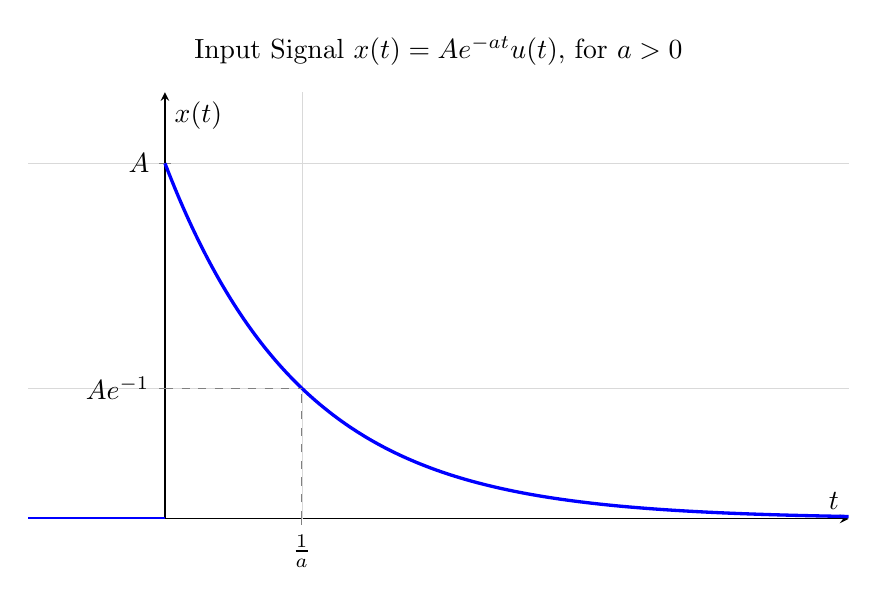
\begin{tikzpicture}
	\begin{axis}[
		width=12cm,
		height=7cm,
		title={Input Signal $x(t) = A e^{-at} u(t)$, for $a>0$},
		xlabel={$t$},
		ylabel={$x(t)$},
		axis lines=middle,
		xmin=-1, xmax=5,
		ymin=0, ymax=1.2,
		xtick=\empty,
		ytick=\empty,
		extra x ticks={1},
		extra x tick labels={$\frac{1}{a}$},
		extra y ticks={0.3678, 1},
		extra y tick labels={$Ae^{-1}$, $A$},
		grid=major,
		grid style={line width=.1pt, draw=gray!30},
		]
		
		% Plot the exponential decay for A=1, a=1
		\addplot[blue, very thick, domain=0:5, samples=200, no marks] {exp(-x)};
		\draw[blue, very thick] (axis cs:-1,0) -- (axis cs:0,0);
		
		% Add guidelines for the time constant
		\draw[dashed, gray] (axis cs:1,0) -- (axis cs:1, {exp(-1)});
		\draw[dashed, gray] (axis cs:0, {exp(-1)}) -- (axis cs:1, {exp(-1)});
		
	\end{axis}
\end{tikzpicture}